%!TEX root = ../../thesis_rui_almeida.tex
\section{DOAS Tomography}%
\label{sec:doas_tomography}

In previous sections (Section~\ref{sec:doas}) we have established that
\gls{DOAS} is a widespread spectroscopic technique with particular usage
in the atmospheric research community. This technique uses either
artificial or natural light to retrieve slant column densities, the
number of molecules that interact with the said light in a given optical
path. These values are described by Equation~\ref{eq:slantColumn}, and
are indeed line integrals.

Also in a previous but different section
(Section~\ref{sec:tomographic_algorithms_and_reconstruction_techniques}),
we have seen that with enough of these integrals (which we can call
projections), we can gather enough information to depict the interior
structure of an object that we make traverse with radiation of some
kind, as long as it is measurable and its behaviour is well known.

Joining the two notions, we can get to the idea that it would be
possible to use \gls{DOAS} in a tomographic manner, so long as we use
sufficient light collection points. This has been proposed by Byer and
Shepp~\cite{Byer1979} in 1979. At the time the authors did not mention
specifically the \gls{DOAS} technique, but the assembly they propose is
essentially equivalent to one that would use this method. \gls{DOAS}
tomography was also mentioned in one of the main pieces of literature in
the field,~\cite{Platt2007}, as one of the most promising avenues
available for \gls{DOAS} progress in the future.

As a requirement for one of the courses that I chose to pursue during
the curricular part of my doctorate, I had to complete an assignment
that consisted in writing a \acrlong{sms} on the subject of \gls{DOAS}
tomography. The study is included in full in Appendix~\ref{ap:tomDoas}.
It aims at characterising the literary panorama regarding the subject
and tries to arrive at a standard application with respect to software,
algorithms and instrumentation.

This type of study has a particular methodology focused on
repeatability. Its complete explanation is out of scope of this section
and even this document, but a simplified schematic is included in
Figure~\ref{fig:sms_schematic}. A more detailed and extensive
description of this method can be found in several works available in
the literature, namely~\cite{Kitchenham2007, Kitchenham2009, Souza2019}.

\begin{figure}[htpb]
    \centering
    \includegraphics[width=.6\textwidth]{img/pdf/sms_planning.pdf}
    \caption{Simplified diagram of the \gls{sms} method. This type of
    study is focused on registering every step of the search and the
    reading  of the retrieved material, in an effort to make the process
    completely repeatable. Adapted from~\cite{Kitchenham2007}.}
    \label{fig:sms_schematic}
\end{figure}

After defining search terms and conducting the actual search, we arrived
at a total of 9 relevant papers. These were analysed under the light of
the study's main goal, which was to identify a standard \gls{DOAS}
tomography device and application.

The first identifiable pattern is the marked prevalence of active
\gls{DOAS} systems. 11 out of the 13 retrieved papers describe or
consider an active \gls{DOAS} system of some kind. As stated in
Section~\ref{sec:doas}, active \gls{DOAS} systems do have better
analytical capabilities than their passive counterparts, although that
comes at the cost of increased instrument complexity and operational
costs. 

Another immediate conclusion is that there is a "dominant" study. Almost
half of the papers found originated from the BABII campaign, in which a
group of researchers set out to quantify pollution through \gls{DOAS}
tomography along a busy German motorway, in the beginning of the
21\textsuperscript{st} century~\cite{Hartl2005, Hartl2006,
Laepple2004, Pundt2005, Pundt2006, Pundt2005a, Mettendorf2005}.

All of the active \gls{DOAS} systems were purposely built for their
corresponding experiment (or group of experiments). BABII researchers
used two telescopes with around 200mm diameter and 1m focal length to
simultaneously illuminate 8 retroreflectors that were assembled onto two
towers located on each side of the road. In one of the papers associated
with this initiative, the same telescope instrumentation was used to
validate the 2D reconstruction technique that was going to be used in
the other papers. The campaign's main assembly is illustrated in
Figure~\ref{fig:babii}.

\begin{figure}[htpb]
    \centering
    \includegraphics[width=0.6\linewidth]{img/png/babii_geometry.png}
    \caption{BABII assembly geometry. In this experiment campaign, the
    telescopes illuminated retroreflecting targets that were positioned
    in two steel towers on both sides of a busy motorway in Germany,
    connecting Heidelberg to Mannheim~\cite{Pundt2005a}.}
    \label{fig:babii}
\end{figure}


Another important initiative with respect to \gls{DOAS} tomography was
the study conducted in 2016 by Stutz et al~\cite{Stutz2016}. The
approach in this case was to use a similar telescope to detect the light
emitted by a narrow interval UV LED light source (290nm) to create a
fence line monitoring system for Benzenes, Toluene and Xylene. The team
managed to apply this system in a successful manner in refineries in Los
Angeles and Houston. One of the most interesting aspects of this study
is that it details a tomographic system that could easily be
commercially deployed.

Another type of \gls{DOAS} tomography system was proposed by researchers
in the Cork Institute of Technology~\cite{ODriscoll2003,ODriscoll2003a,
Murphy2003}.  In their three papers, the authors describe \textbf{1)} a
new multipath instrument that significantly increases the amount of
projection information in this kind of application; \textbf{2)} a
tomographic reconstruction algorithm based on evolutionary algorithms;
and \textbf{3)} the application of \gls{DOAS} tomography to a simulated
urban canyon scenario. Although all three papers present technological
innovation, it would not be fair not to say that from a strictly
literary point of view, these were among the weakest retrieved by the
search process.

Regarding passive DOAS applications, the two papers we have found come
with two completely different paradigms. The first
article~\cite{Johansson2009} was written in 2009 and details the
application of a tomographic inversion algorithm to a scanning DOAS
application, designed to work with trace gas plumes like the ones above
volcanoes or power stations. The team present a system composed of two
DOAS devices, with sufficient distance with themselves as to allow
tomographic reconstruction, but sufficiently small to allow the light
path to be considered a straight line from the point of last scattering
to the detector. The authors applied an adapted version of the Lower
Third Derivative (LTD) algorithm to the projections obtained by pointing
the set of fixed DOAS apparatus towards the plume in different angles.
Besides simulations for their proposed method, the authors have also
conducted practical experiments, both over a power plant in Spain and a
volcano in Italy. Results from these experiments display a good
agreement between reality and simulation results, proving the
technique's validity.

The second Passive DOAS application is a paper published by Frins et
al.~\cite{Frins2006}. In this study, the researchers detail a particular
application in which they measure light coming from bright and
nonreflecting sun-illuminated objects in their field of view. They use
this light to retrieve column density values for a number of trace
gases. The proposed method also includes a way with which to remove the
stratospheric contribution that appears in the measured light besides
the target column. The authors discuss how radiative transfer can
influence measurements, but they also present a number of approaches to
mitigate this problem, ensuring the validity of their approach.  Besides
presenting the method, the authors also describe an experiment they
conducted by assembling and manoeuvring a DOAS system on top of a
building in Heidelberg, Germany.

\begin{figure}[htpb]
    \centering
    %left bottom right top
    \begin{subfigure}[b]{.475\textwidth}
        \centering
        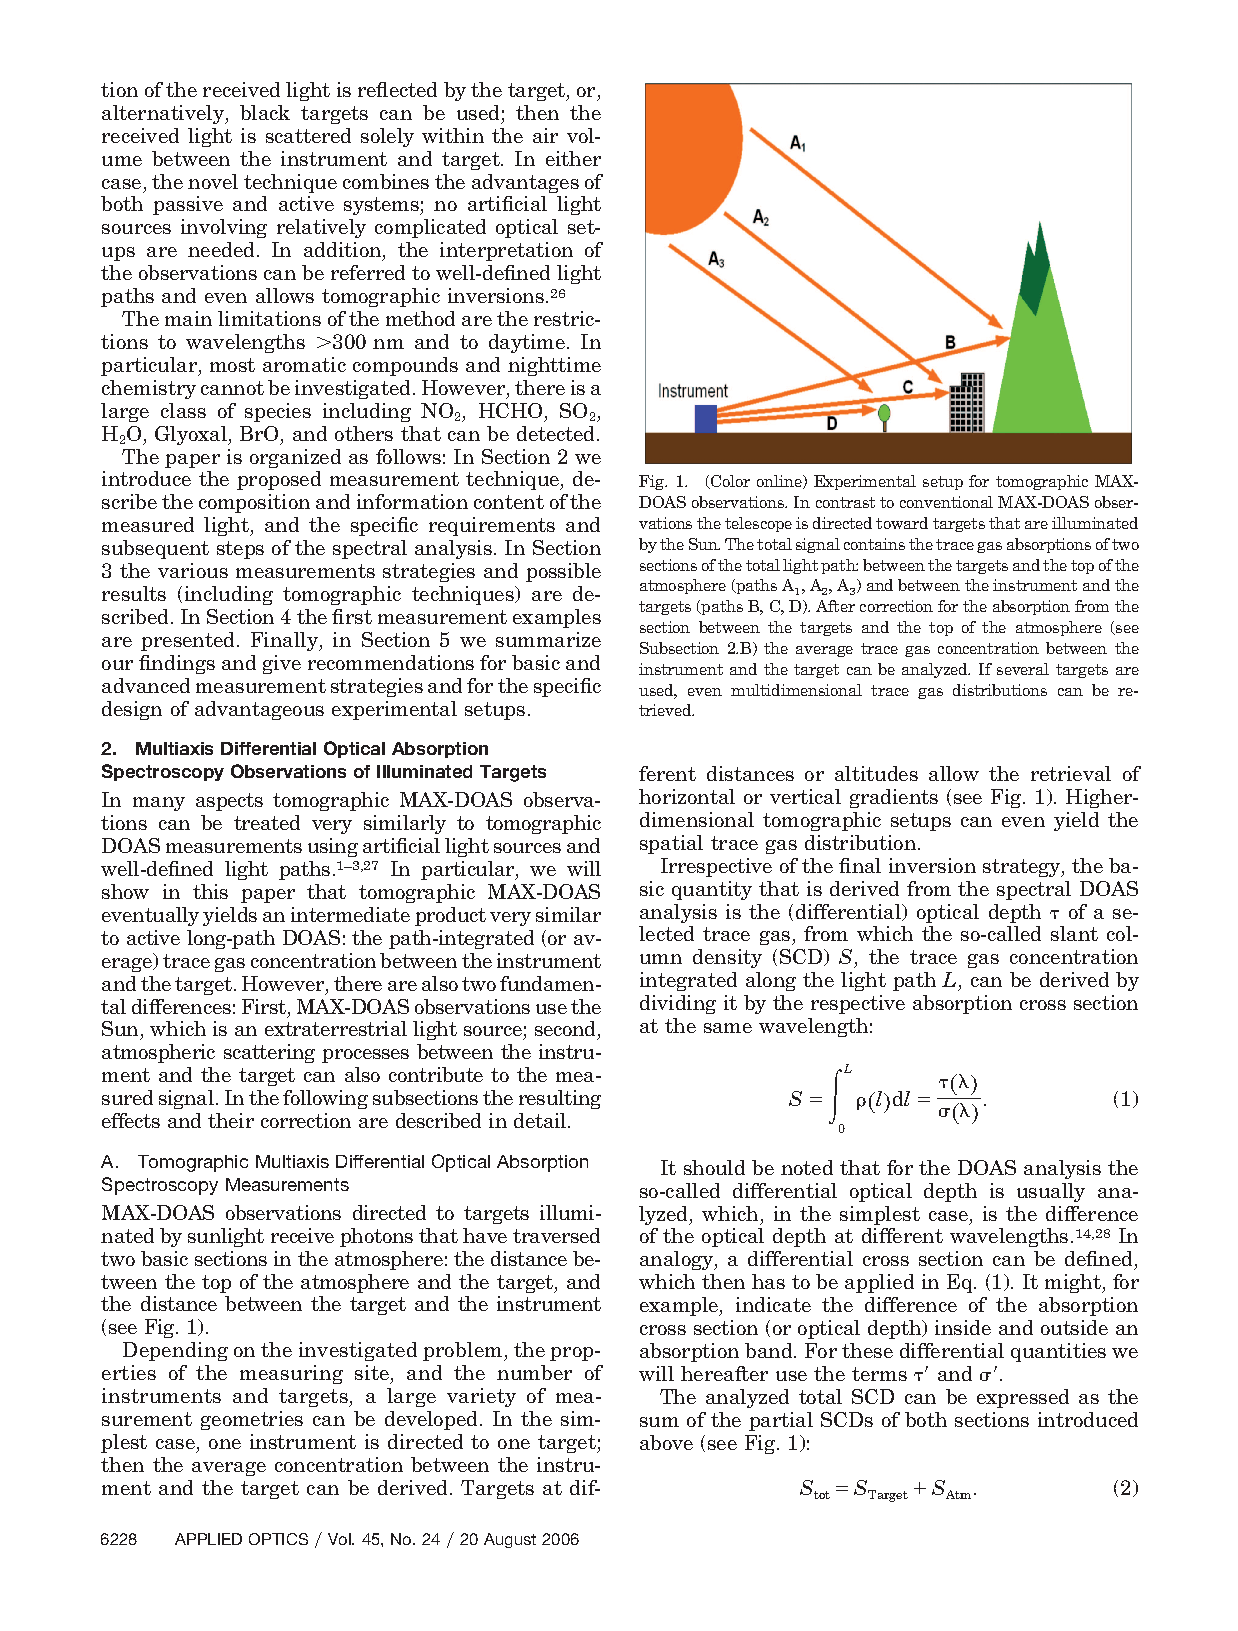
\includegraphics[trim=10.8cm 19.7cm 2cm 2cm, clip, %...
        width=\textwidth]{img/pdf/frinsSchematics_p2.pdf}
        \caption{Schematic representation of Frins's
        assembly~\cite{Frins2006}.}
        \label{fig:frins_schem_1}
    \end{subfigure}
    \hfill
    \begin{subfigure}[b]{.475\textwidth}
        \centering
        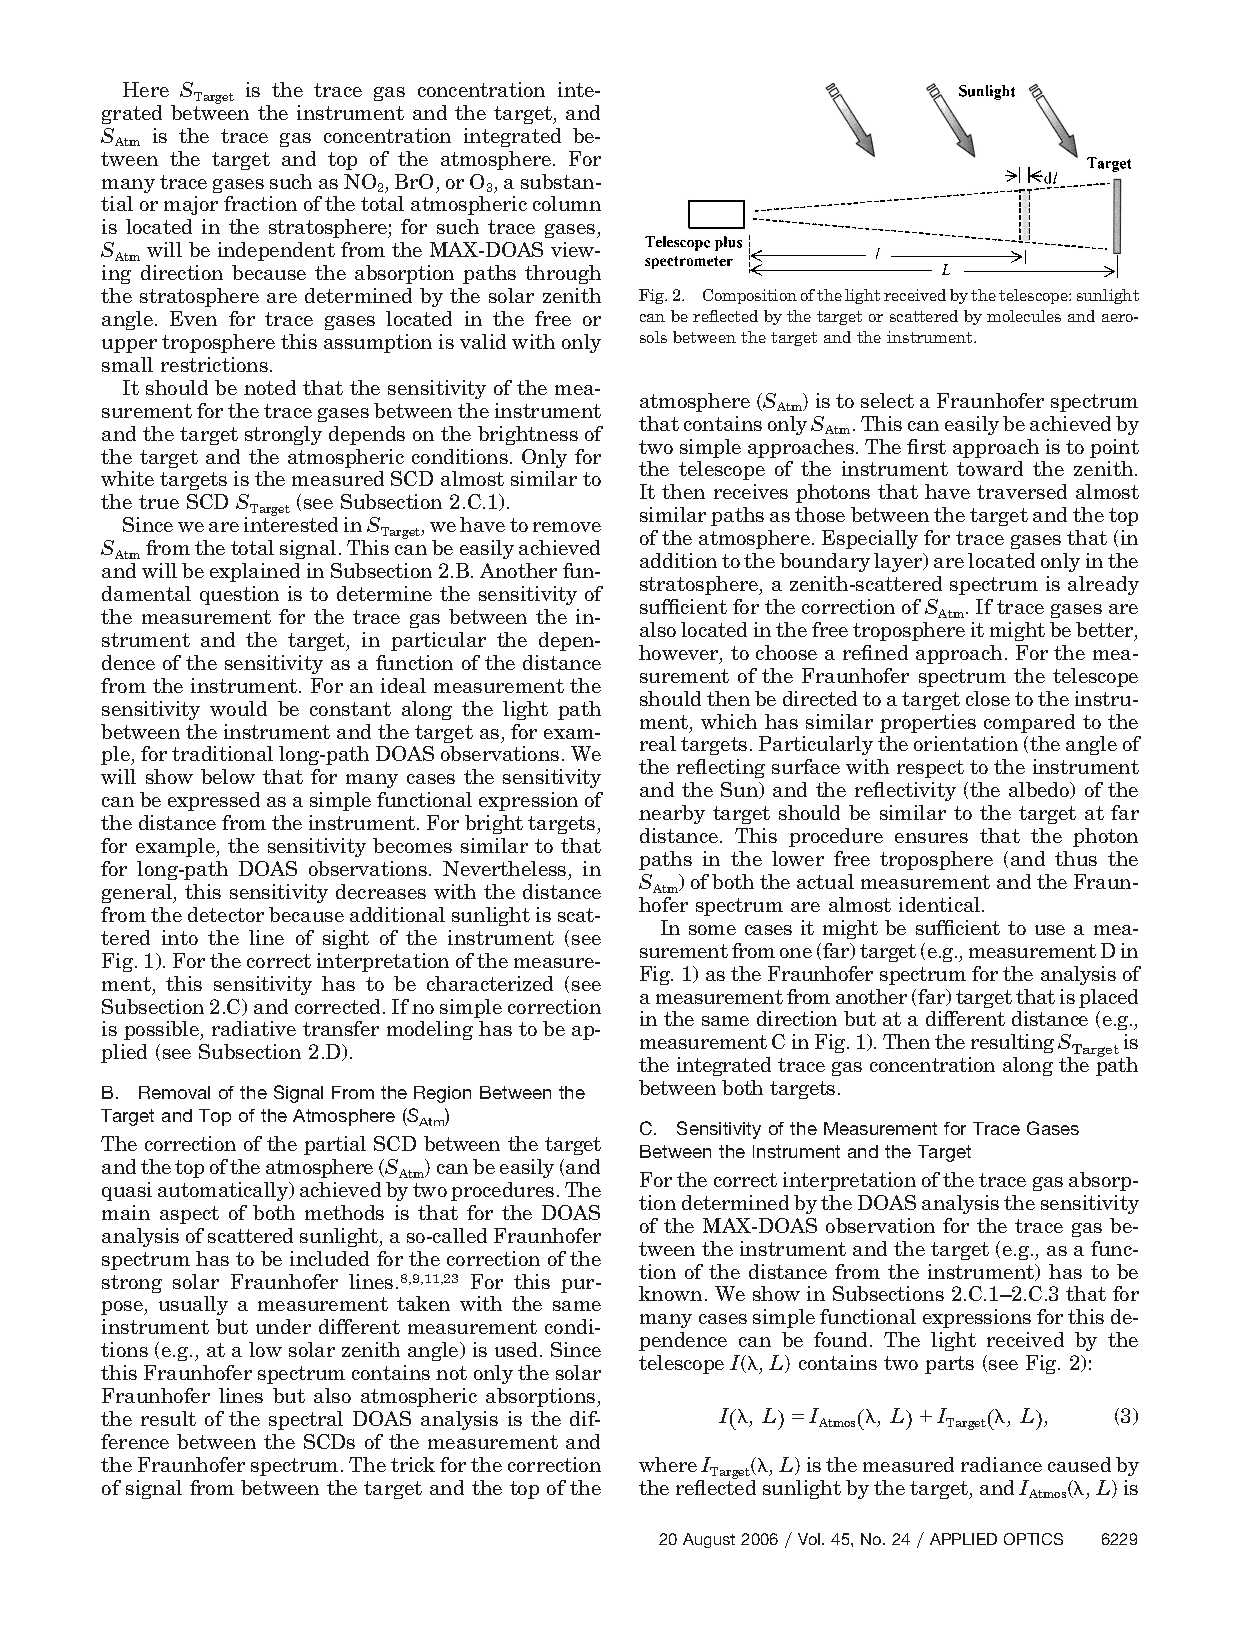
\includegraphics[trim=10.8cm 22.8cm 1cm 1cm, clip, %...
        width=\textwidth]{img/pdf/frinsSchematics_p3.pdf}
        \caption{The physical principle behind Frins's
        paper~\cite{Frins2006}.}
        \label{fig:frins_schem_2}
    \end{subfigure}
    \caption{Erna Frins's paper~\cite{Frins2006} proposes a very
        relevant passive \gls{DOAS} application that can conceptually be
        employed in a \gls{DOAS} tomography scenario. In this 2006
        paper, the authors use multi-axis measurements of
        sun-illuminated targets to estimate absorption paths without
        using radiative transfer models.}
    \label{fig:ernafrins}
\end{figure}

In summary, the search has found that active tomographic \gls{DOAS} is
far more common than the passive counterpart (11 out of 13 articles
discussed this method). This preference can be explained by the fact
that the results produced by this kind of system are generally superior
to those obtained by passive methods. However, passive applications are
normally much less demanding on a technical level, and are simpler to
run and assemble.  Much as a result of this, we have also identified
that the systems used in the literature were not mobile or had a very
low mobility level which in turn caused that all the systems were
working with low projection numbers. This should be taken into account
in future research on the topic. As a final note, we would also like to
point out that there is no commercially available systems for this kind
of application, although some of the articles, like the one by Stutz in
2016~\cite{Stutz2016} detail systems which could easily be adapted to
that end.
